In the Feasibility Study of the our Project Initiation we already discussed some structure of the output. In general, our output will be a set of graphs depicted in different views. One of these views will be the original view that is computed from the log file directly. Nodes in this graph represent states in the logs. Each node contains the name of the state, the average duration and the total number of occurrences in the event log. The average is computed over all occurrences.
The edges represent state transitions. When in a trace, one state directly follows another one then their corresponding nodes are to be connected by a directed edge where this edge points to the later, successor state. Each such transition is annotated with the relative frequency of transitions to the target state given the total number of occurrences from that state \textbf{or the total number of outgoing transitions from that state}. This is illustrated in Figure \ref{fig:ogview}.

\begin{figure}[htbp]
    \centering
    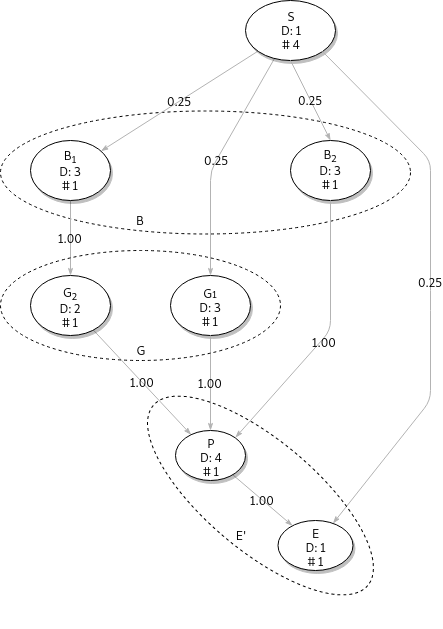
\includegraphics[width=0.7\textwidth]{../Diagrams/Statecharts/statemachine.png}
    \caption{An example output following the log presented above. We see that the transition from $S$ to $B_1$ is annotated by the numeric value $0.25$. This follows from that fact that $B_1$ followed $S$ in a fourth of the times. The dashed ellipses represent a possible view on could choose.}
    \label{fig:ogview}
\end{figure}

The other output graphs correspond to the views as specified in the subsection on the input. In a view, a number of states can be lumped into the same state. In the above example view 1, the states $B_1$ and $B_2$ are combined to the state $B$. The resulting state holds again an average duration time. We imagine two different possibilities for the computation of this value. Either we could average over all occurrences of every state in the combined state or for every trace sum up the total duration time in the combined state and then average over all traces\footnote{We deem the latter option to be more meaningful but leave the discussion to be open until our advisor has been consulted about this issue.}. The total number of occurrences of the composite state is the sum of the number of occurrences of every component state. 



We shall investigate the transition frequencies of the composite states further. Let $\Omega$ denote the state space. We consider a transition from the composite states $S \subset \Omega$ to $T \subset \Omega$ where we understand both states as sets of basic states. The number of transitions from states all substates of $S$ to all substates of $Q$ is then the number
\[ 
    \sum_{(s,q) \in S \times Q} N(s,q)
\]
where $N(s,q)$ denotes the number of transitions observed between the original, raw states $s$ and $q$. The relative frequency of transitions between the composite states $S$ and $Q$ is then given by the above sum divided by the number
\[
    \sum_{(s,t) \in S \times \Omega} N(s,t)
\]
of outgoing transitions from the lumped state $S$.

To illustrate this procedure let us consider the partitioning chosen in figure \ref{fig:ogview}. Here a we have the state space $\Omega = \{ S, B_1, B_2, G_1, G_2, P, E \}$\footnote{Mind that $S$ is here a basic state while in our notation about $S$ is composite}. The composite states we chose in the first example view are $B := \{ B_1, B_2 \} $, $G = \{ G_1, G_2 \}$ and $E' = \{ P, E \}$. The graph is then transformed according to the rules discussed above, yielding the graph in figure \ref{fig:view1}.

\begin{figure}[hb]
    \centering
    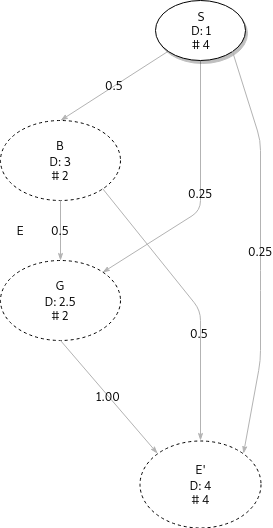
\includegraphics[width=0.5\textwidth]{Diagrams/Statecharts/statemachine_view1.png}
    \caption{State composition of figure \ref{fig:ogview} has been applied and the transitions and state informations adjusted according to the rules discussed in the text.}
    \label{fig:view1}
\end{figure}

Another example for how a view is supposed to transform the graph we can find in figure \ref{fig:pandv}.

\begin{figure}[H]
    \centering
    \begin{subfigure}[b]{0.6\textwidth}
        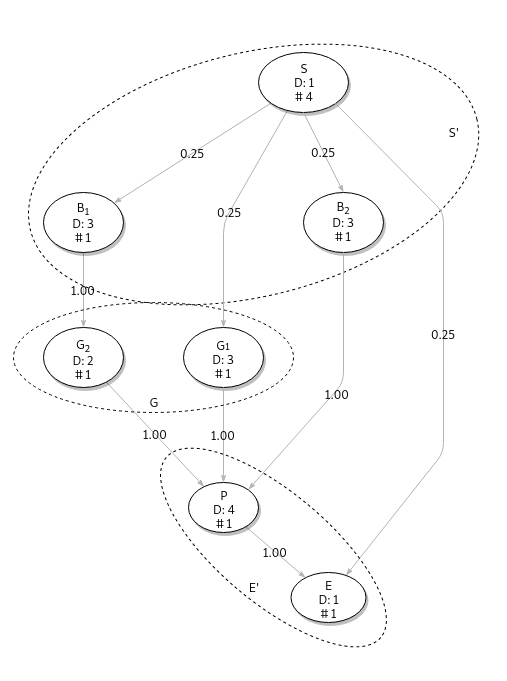
\includegraphics[width=\textwidth]{Diagrams/Statecharts/statemachine_preview2.png}
        \caption{State chart with a different partitioning of states.}
        \label{fig:preview2}
    \end{subfigure}
    \\ %add desired spacing between images, e. g. ~, \quad, \qquad, \hfill etc. 
      %(or a blank line to force the subfigure onto a new line)
    \begin{subfigure}[b]{0.45\textwidth}
        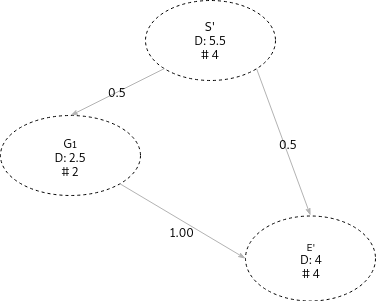
\includegraphics[width=\textwidth]{Diagrams/Statecharts/statemachine_view2.png}
        \caption{The resulting view.}
        \label{fig:view2}
    \end{subfigure}
    \caption{A different selection of composite states in the same example and the requirement for the output graph.}
    \label{fig:pandv}
\end{figure}